%Introduction



\section{Introduction}
Today's applications are increasingly stored in the cloud for more flexibility and scalability. However, the environment cloud providers provide is not secure, due to it being vulnerable to attacks, where customers' data can be stolen. More detailed, reasons to consider the cloud as untrustworthy are (1) poor administration, (2) vulnerabilities of the software stack, or (3) missing encryption of the data.
  That is, finances and health applications that handle sensitive data cannot afford this risk by hosting their applications on the cloud. To make cloud infrastructure more reliable even for such fields with high security requirements, confidential computing has become a new trend.\\
 A CCS is an additional service that can be applied on top of an existing cloud provider~\cite{confidentiality}. These confidential services are needed when services have high security requirements, which cannot be guaranteed by a normal cloud provider. As the cloud provider or its administration cannot be trusted either, the sensitive data must also be protected from this provider itself. \\
 The three properties data confidentiality, integrity protection, and high availability, short CIA, build a triad,  shown in Figure~\ref{cia},  that describes three important requirements of information security~\cite{ciaBook, cia}. It contains data Confidentiality, Integrity Protection, and High Availability.\\
 Data confidentiality is keeping the data private, which is very important, especially for cloud providers. Challenges are encrypting the data and protecting the encryption keys.\\
 Integrity protection is the insurance of complete and correct code that is not changed by a bad party. Accordingly, it can be considered a prerequisite for confidentiality. But these two characteristics are hard to implement although they are mandatory for cloud computing. Indeed, the cloud computing TCB  is considered huge as it includes the cloud providers and their infrastructure, so applications in the field of finances, medicine, or governmental issues cannot afford to trust this whole TCB.\\
 High availability is required by the fact that people rely on the systems that are on the cloud. Accordingly, they should work, even if failures occur.\\
 Another problem confidential cloud services should handle is every kind of attack. Especially in the cloud, where you cannot even trust the provider, many attacks can happen, above all on big cloud providers. Therefore it is mandatory to detect and protect against such attacks like forking attacks, physical attacks, or rollback attacks.\\
 This paper introduces two different CCSs, the Confidential Consortium Framework (CCF)~\cite{Howard} and Nimble~\cite{Nimble}. CCF is a framework for multiparty applications that provides confidential computing on the cloud. Nimble is a service that detects and prevents rollback attacks in addition to also providing confidentiality. I present the design of both systems and discuss their advantages and disadvantages.
	 
 \begin{figure}[t]
	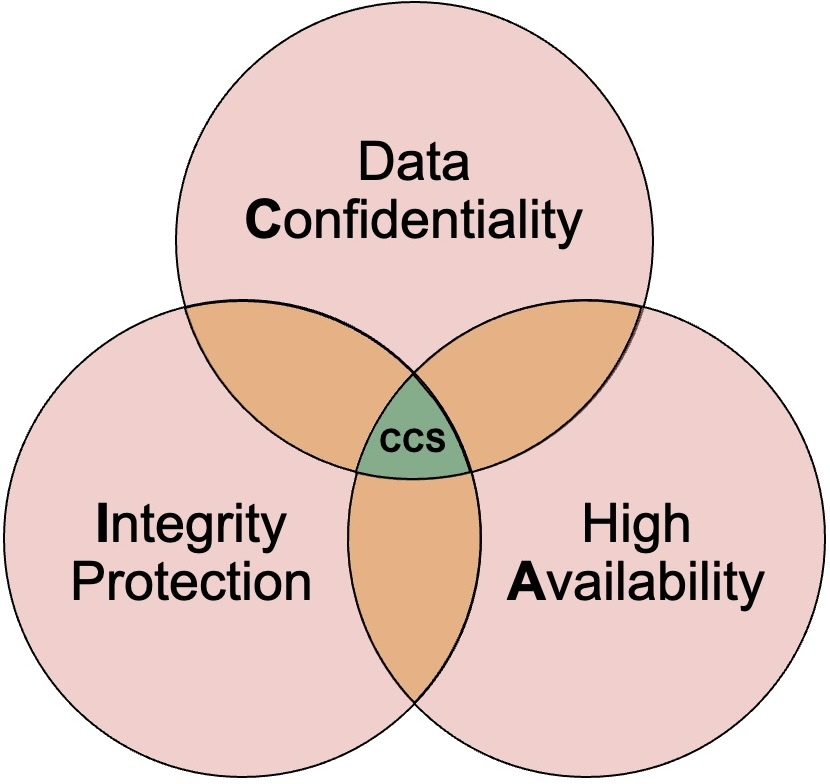
\includegraphics[scale=0.17]{pictures/cia_new}
	\caption{The CIA triad, consisting of the three properties Data Confidentiality, Integrity Protection, and High Availability, each represented as a circle. A Confidential Cloud Service (CCS) aims to realize all three CIA properties which is the intersection of all circles in the figure.  }
	\label{cia}
\end{figure}